\section{Introduction}

The efficacy of arbitrary order Volterra-Laguerre MPC, proposed in Chapter \ref{chap:10}, will be assessed in this chapter through two application examples relevant to the process industries. In each example, the considered problem is control of the fluid level in a nonlinear system of connected water tanks. In such systems, the nonlinear dynamics arise due to Bernoulli's principle, which dictates the flow of water through valves \cite{Batchelor2000}. Additionally, constraints exist on the input due to saturation, and at the output to prevent overflow.

The first application example is based on the cascaded tanks benchmark system from Chapter \ref{chap:6}, which is investigated in this chapter via an accurate state space model simulation. Practical implementation of the MPC method is then considered in the second example; a physical system of horizontally coupled tanks with optional disturbance pump in the output tank. In both test applications, the performance of the proposed Volterra-Laguerre MPC is assessed and compared against existing MPC methods using linearized or simplified model structures. In the practical example, the effect of the prediction horizon on reference tracking and disturbance rejection is experimentally verified.

\section{Simulation study on the cascaded tanks}
\label{sec:CascadedTanksMPC}

We return to the cascaded tanks benchmark system, introduced in Chapter \ref{chap:6}, to motivate our first MPC application example. A schematic overview of the system setup can be found in Figure \ref{fig:System_Tanks}, where $u(t)$ and $y(t)$ will become the control input and output respectively. The results in Section \ref{sec:Results_tanks} revealed that a second order Volterra-Laguerre model can provide accurate predictions for the dynamics of the cascaded tanks. In this section, the system will be examined through simulation only, with new Volterra series models being identified prior to the control experiment. The proposed MPC algorithm will be compared against the method proposed in \cite{Parker1998} for second order Volterra-Laguerre models, as well as a linear MPC scheme.

\subsection{Experiment methodology}

In order to simulate the cascaded tanks system, we employ a nonlinear continuous-time state space model developed in \cite{Pan2018}, whose parameters have been estimated using the real benchmark data. For simplicity, we will neglect the possibility of having process noise, measurement noise or tank overflow, such that the model can be described by,
\begin{align}
\dot{x}_1 &= -k_1 \sqrt{x_1} + k_4 u, \\
\dot{x}_2 &= k_2 \sqrt{x_1} - k_3 \sqrt{x_2}, \\
y &= 0.5(x_2 - L),
\end{align}
where $x_1$ and $x_2$ are the water levels (in cm) of the upper and lower tanks respectively, $L$ is the length of the valve, $u$ is the pump input (in V), $y$ is the output water level (in V), and $k_1, k_2, k_3, k_4$ are the estimated parameters. The pump is unidirectional, such that the input voltage ($u$) cannot be negative.

The simulation model is first used to perform an identification experiment, where $8000$ samples of input/output data are collected. The input is designed as a filtered noise sequence which ranges between 0 and 8V, such that the output moves through the entire range of intended operating levels. Two second order Volterra-Laguerre models are identified for the tanks system, using the same method employed in Chapter \ref{chap:6}, i.e. the regularized basis function approach (ReLBF) proposed in Chapter \ref{RegBFs_Chap5}. The first model takes full advantage of the flexible state space structure, (\ref{eqn:SS_dynamic_VL}) and (\ref{eqn:SS_output_VL}), developed in the previous chapter, with separate Laguerre bases at each order and a constant $\alpha_0$ kernel. The second model uses the simplified structure imposed in \cite{Parker1998}, where each nonlinear order uses the same Laguerre basis and the constant kernel is neglected. 

To assess the control performance of the MPC approach proposed in this thesis, the following control methods are applied to the simulated tanks system:
\begin{enumerate}
\item \textbf{Proposed:} MPC using Algorithms \ref{alg:BasicVL-MPC}, \ref{alg:ConstrainedVL-MPC} and a full Volterra-Laguerre model with constant kernel and unique Laguerre bases ($\mathcal{B}_1 = 15$, $\mathcal{B}_2=10$). 
\item \textbf{Simplified:} MPC using Algorithms \ref{alg:BasicVL-MPC}, \ref{alg:ConstrainedVL-MPC} and the simplified Volterra-Laguerre structure ($\mathcal{B}_1 = \mathcal{B}_2 = 15$, $a_1=a_2$, $\alpha_0=0$) used in \cite{Parker1998}. 
\item \textbf{Linear:} Linear MPC using the MATLAB 2018a Model Predictive Control toolbox and a linearized plant model around a $y=5V$ operating point.
\end{enumerate}
The applied reference signal is chosen to be a step sequence covering the full output range. For the linear MPC method, the linearized model is obtained directly from the nonlinear state equations. The prediction horizon is $p=50$ for all methods, and the move horizon is $\mu=1$, with sampling period fixed at $4$ seconds. The input penalty scaling is set as $\Gamma_u = 1$ in Algorithm \ref{alg:BasicVL-MPC}.

\subsection{Volterra-Laguerre model estimates}

For the full unsimplified model, the first and second order Volterra-Laguerre kernels are shown in Figure \ref{fig:ProposedKernels_MPC}, and the constant contribution is estimated as $\alpha_0 = -6.59$. Note that the estimate for $\alpha_0$ results from the series expansion of a nonlinear state space model, and could not have been determined and corrected for using prior system knowledge. The Laguerre poles chosen by the optimization routine are also found to be significantly different, with $a_1 = 0.80$ and $a_2 = 0.45$.

\begin{figure}[h]
\centering
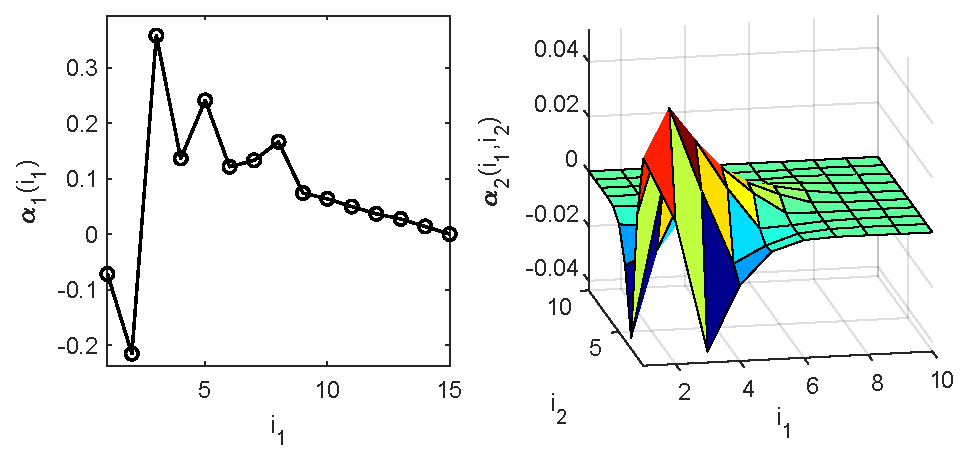
\includegraphics[width=0.85\textwidth]{Chapter11_ControlStudy/Alternate0_kernels_coloured.pdf}
\caption{Cascaded tanks Volterra-Laguerre kernel estimates for the proposed method}
\label{fig:ProposedKernels_MPC}
\end{figure}

For the simplified model, the two kernels are given in Figure \ref{fig:SimplifiedKernels_MPC}, with $\alpha_0$ neglected. Using only a single Laguerre basis, the optimized pole location is $0.68$; a clear compromise between the two optimal pole locations estimated in the full model.

\begin{figure}[h]
\centering
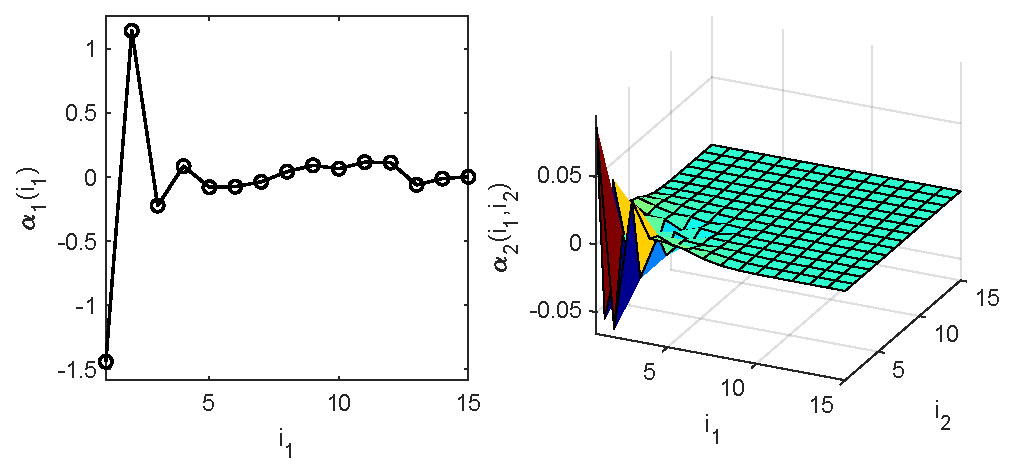
\includegraphics[width=0.85\textwidth]{Chapter11_ControlStudy/Simple_kernels_coloured.pdf}
\caption{Cascaded tanks Volterra-Laguerre kernel estimates for the simplified method}
\label{fig:SimplifiedKernels_MPC}
\end{figure}

\subsection{MPC results}

For a sequence of step changes applied to the reference, the controlled outputs for each method are shown in Figure \ref{fig:p50_comparison_MPC}, while the corresponding MPC-computed inputs are given in Figure \ref{fig:p50_inputs_MPC}. It is clear from the output response that the simplified Volterra-Laguerre structure does not give satisfactory control performance, with slower settling times and large steady state errors at lower water levels where the nonlinearities are strongest. This can be attributed to the inability of such a constrained model structure to properly capture the dynamics of the nonlinear system. In contrast, the proposed method gives good dynamic and steady state performance for every step change. 

\begin{figure}[h]
\centering
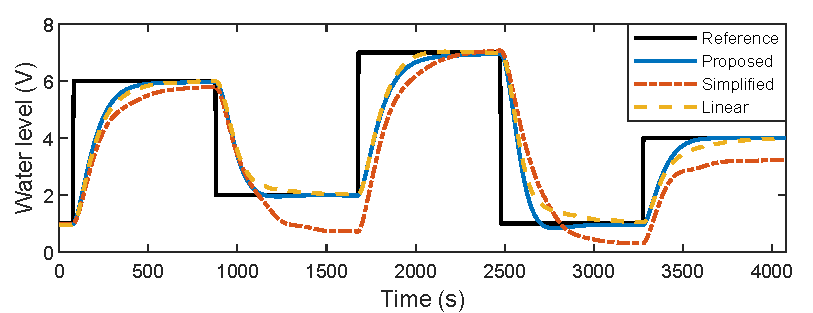
\includegraphics[width=0.8\textwidth]{Chapter11_ControlStudy/p50_equalPenalty_outputs.pdf}
\caption{Step sequence reference tracking comparison}
\label{fig:p50_comparison_MPC}
\end{figure}

\begin{figure}[h]
\centering
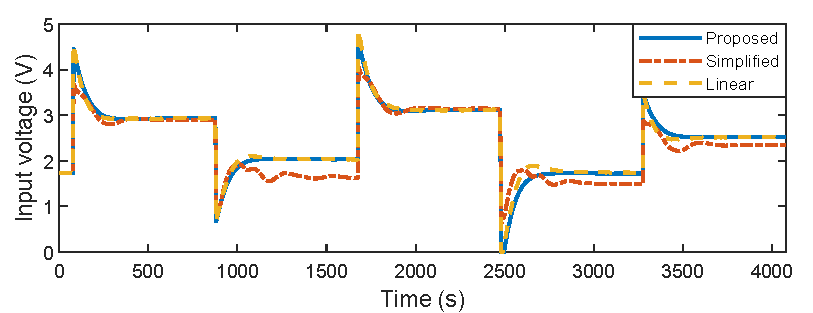
\includegraphics[width=0.8\textwidth]{Chapter11_ControlStudy/p50_equalPenalty_inputs.pdf}
\caption{MPC inputs for step sequence reference}
\label{fig:p50_inputs_MPC}
\end{figure}

Comparing the proposed method with the linear MPC approach, it can be seen that the performance is comparable for high water levels, but when the water level measurement drops as low as $1$V in the latter half of the record, there is a noticeable degradation in the linear MPC settling times. This result is not surprising, as the fluid dynamics will be most strongly nonlinear when the water level is very close to the exit valve, and thus there will be large deviations from the linearized model obtained from the mid-level of the tanks. The linear model does, however, provide far better results than the simplified Volterra-Laguerre model, and this is due to the use of an exact linearization rather than attempting to estimate nonlinear dynamics over the full tank range without enough model flexibility.

Furthermore, to illustrate the constraint handling performed by Algorithm \ref{alg:ConstrainedVL-MPC}, the MPC objective function is plotted, for the proposed method, at two important instances. Figure \ref{fig:ImpossibleGlobalMin_MPC} plots the objective function immediately following the first positive reference step. Here we see the global minimum being rejected for violating an input constraint, and from the remaining candidates, the positive local minimum is chosen for implementation. Figure \ref{fig:ImpossibleGlobalMin_negativestep_MPC} shows the objective function output directly following the second negative reference step, which also features a global minimum outside of the constrained region. In this case, however, there are no stationary points inside the constraint, and so the constraint boundary is chosen for implementation. This can be observed in Figure \ref{fig:p50_inputs_MPC} (at $2500$s), where the input briefly sits at the $0$V boundary.

\begin{figure}[h]
\centering
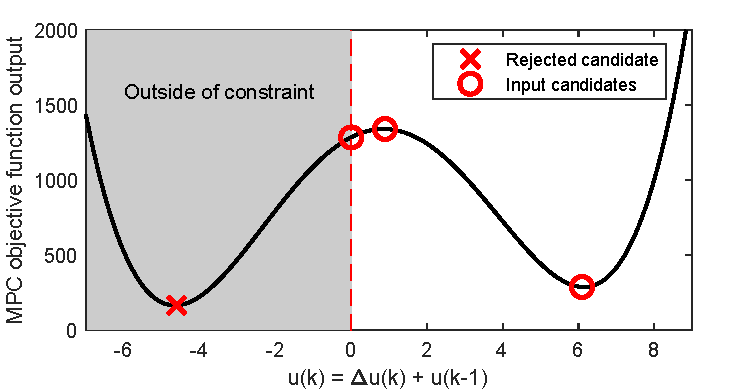
\includegraphics[width=0.7\textwidth]{Chapter11_ControlStudy/ImpossibleGlobalMin.pdf}
\caption{Objective function cost after the first positive reference step}
\label{fig:ImpossibleGlobalMin_MPC}
\end{figure}

\begin{figure}[h]
\centering
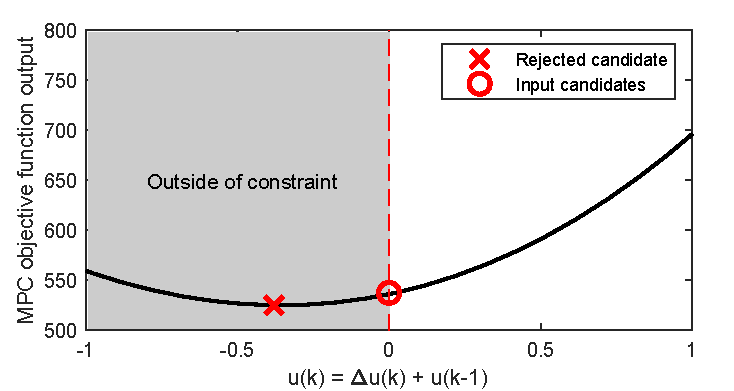
\includegraphics[width=0.7\textwidth]{Chapter11_ControlStudy/ImpossibleGlobalMin_negativestep.pdf}
\caption{Objective function cost after the second negative reference step}
\label{fig:ImpossibleGlobalMin_negativestep_MPC}
\end{figure}

\section{Physical test on a coupled tanks apparatus}

For the second application example, we move from simulation to practice, by evaluating the proposed MPC scheme on a physical system of coupled water tanks. The configuration of the physical apparatus, shown in Figure \ref{fig:CoupledTanksSchematic}, is similar in nature to the benchmark system considered in Section \ref{sec:CascadedTanksMPC}, except that the movement of water from the first to the second tank is now facilitated by a horizontal valve. There is also potential for adding process disturbances via a second pump into the output tank. This section presents results on model identification, water level control and disturbance rejection for the coupled tanks, using the methods proposed in this thesis. 

\begin{figure}[h]
\centering
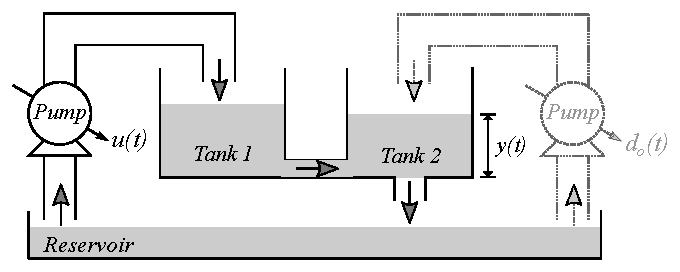
\includegraphics[width=1\textwidth]{Chapter11_ControlStudy/CoupledTanksSchematicDisturbance.pdf}
\caption{Schematic overview of the water flow dynamics in the coupled tanks test apparatus}
\label{fig:CoupledTanksSchematic}
\end{figure}

\subsection{Experiment methodology}

In the identification stage, the excitation input, $u(t)$, to the pump is filtered Gaussian noise ranging between 1.5 and 5.5V, such that the sensor output $y(t)$ in the second tank varies over its full range of 0 to 7V. Data is collected at a sampling period of $T_s = 10s$, with $8080$ samples collected from the input and output and split into two equal parts to produce the estimation and validation datasets shown in Figure \ref{fig:CoupledTanksData}. 

\begin{figure}[h]
\centering
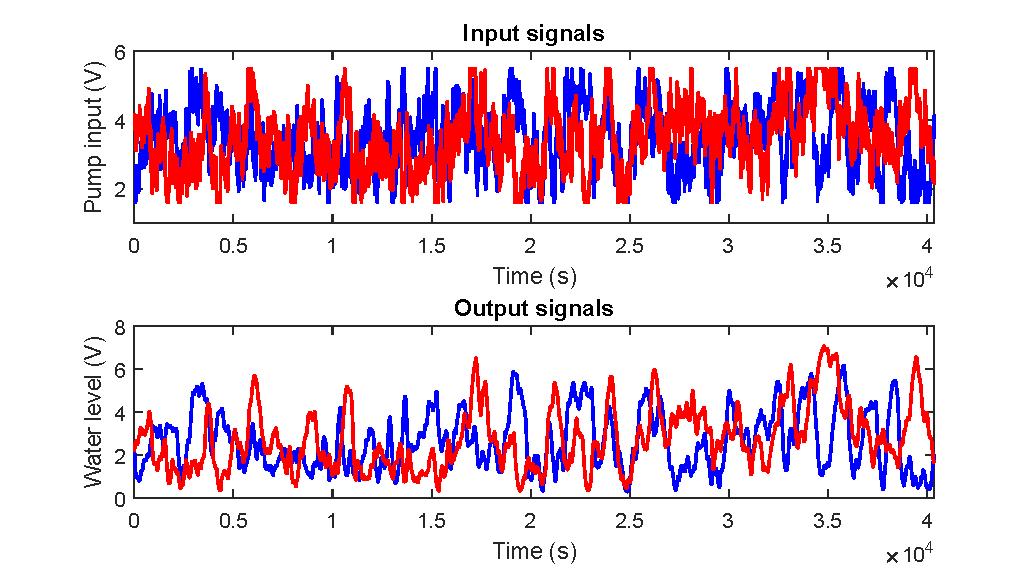
\includegraphics[width=1\textwidth]{Chapter11_ControlStudy/CoupledTanksDatasets.pdf}
\caption{Estimation (blue) and validation (red) datasets for identification of the coupled tanks apparatus}
\label{fig:CoupledTanksData}
\end{figure}

Three Volterra-Laguerre models are identified and validated using the data: linear, 2\textsuperscript{nd} order and 3\textsuperscript{rd} order. The linear model contains only the 1\textsuperscript{st} order LBF kernel (no constant offset), while the latter two models contain every kernel up to the maximum order considered. The models are estimated using the regularized basis function method (ReLBF) proposed in Chapter \ref{chap:5}, where separate Laguerre poles are identified for each kernel.

After obtaining the model estimates, the linear and 3\textsuperscript{rd} order models are used to test the performance of the proposed Volterra-Laguerre MPC in Chapter \ref{chap:10}. More specifically, control is applied to the tanks for each model using Algorithms \ref{alg:BasicVL-MPC}, \ref{alg:ConstrainedVL-MPC} and the disturbance model technique in Section \ref{sec:DisturbanceModel_MPC}. The input penalty is set to $\Gamma_u = 0$ as the penalty is not required for stablity of the closed loop system. Evaluation of the control performance is conducted using the following experiments:
\begin{enumerate}
\item Reference tracking comparison of linear and 3\textsuperscript{rd} order Volterra-Laguerre MPC using a step sequence reference and prediction horizon $p=25$
\item Step response comparison for varying prediction horizons in the 3\textsuperscript{rd} order Volterra-Laguerre MPC
\item Disturbance rejection comparison for varying prediction horizons in the 3\textsuperscript{rd} order Volterra-Laguerre MPC
\end{enumerate}
In the third experiment, the disturbance, $d_o(t)$, is a pulse from 0 to 2V and of width 1500s, which is applied to the disturbance pump shown in Figure \ref{fig:CoupledTanksSchematic} (dotted lines).

\subsection{Identification results}

For each of the models identified using the estimation data, prediction accuracy is assessed using the RMS validation metric (\ref{eq:e_RMSt}), i.e.
\begin{equation}
e_{RMSt} = \sqrt{\frac{1}{N_v} \sum_{t=1}^{N_v} (y_{mod}(t) - y_v(t) )^2},
\label{eq:e_RMSt_MPC}
\end{equation}
where $y_v$ is the validation output of length $N_v$, and $y_{mod}$ is the modeled output for the same validation input.

The errors for each identified model are reported in Table \ref{tab:CoupledTanksVal}. The linear model is seen to be a relatively poor predictor of system behaviour, while the nonlinear Volterra-Laguerre models have much higher accuracy. The 3\textsuperscript{rd} order model is observed to be the best fit as it exhibits a noticeable 28\% decrease in validation error over the 2\textsuperscript{nd} order model. 

\begin{table}[h]
\centering
\caption{Validation metrics for each Volterra-Laguerre model of the coupled tanks}\label{tab:NRMSE_CED}
\begin{tabular}{|c||c|c|c|}
\hline
\textbf{Model} & Linear & 2\textsuperscript{nd} order & 3\textsuperscript{rd} order \\
\hline
\textbf{$e_{RMSt}$} & 0.6371 & 0.0634 & 0.0457 \\
\hline
\end{tabular}
\label{tab:CoupledTanksVal}
\end{table}

For the 3\textsuperscript{rd} order model, the basis function kernel estimates $\hat{\alpha}_1$ and $\hat{\alpha}_2$ are plotted in Figure \ref{fig:CoupledTanksKernels}, and $\hat{\alpha}_0 = 0.774$. The Laguerre pole locations are $a_1 = a_2 = 0.85$ and $a_3 = 0.50$.

\begin{figure}[h]
\centering
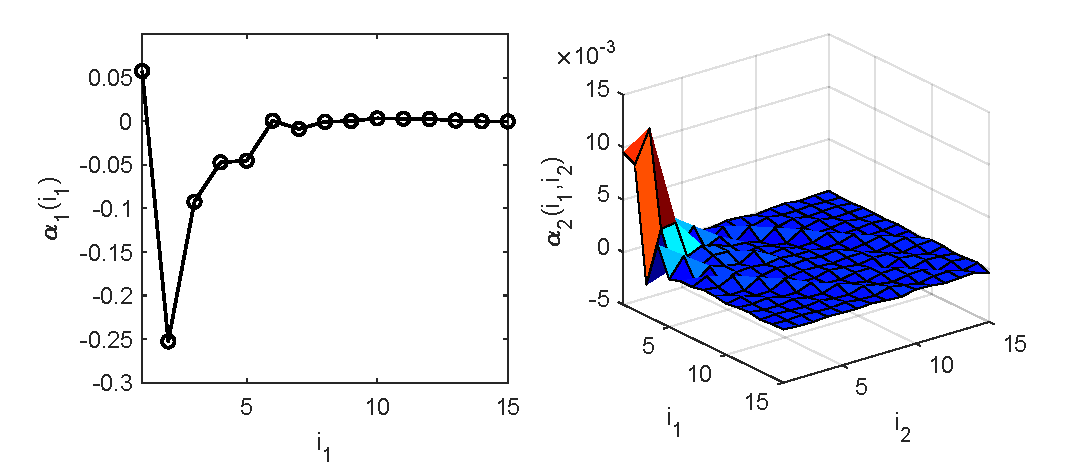
\includegraphics[width=0.9\textwidth]{Chapter11_ControlStudy/CoupledTanks3rdOrderKernels.pdf}
\caption{Basis function kernel estimates for the 3\textsuperscript{rd} order Volterra-Laguerre model of the coupled tanks}
\label{fig:CoupledTanksKernels}
\end{figure}

\subsection{MPC results}

\subsubsection{Reference tracking comparison}

For a step sequence reference signal and $p=25$, the MPC output results are shown in Figure \ref{fig:CoupledTanksStepSequence}. The linear model does not produce desirable control performance, with large overshoots and settling times on most of the reference steps. This result is not surprising given the high validation errors observed for the model in the identification stage, and suggests that a nonlinear model is required for high performance control. The results for the 3\textsuperscript{rd} order model are significantly better, with a desirable response to all of the reference steps. The nonlinear model provides a good characterization of the system dynamics over the entire range of the tank, and MPC could be applied efficiently using the methods of Chapter \ref{chap:10}.

\begin{figure}[h]
\centering
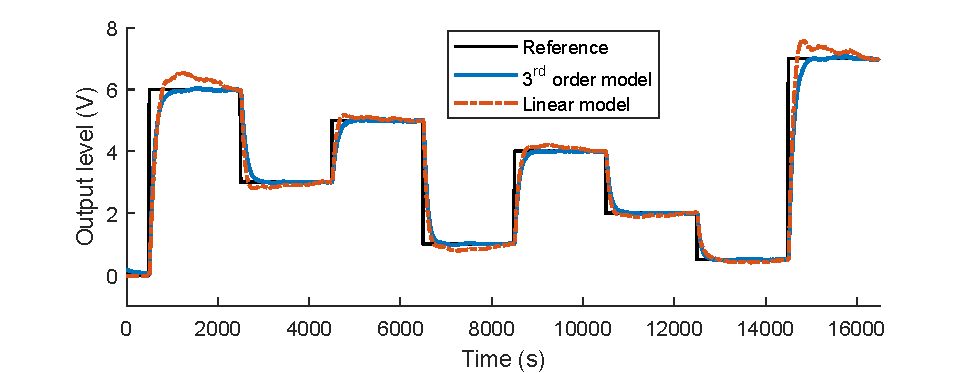
\includegraphics[width=1\textwidth]{Chapter11_ControlStudy/CoupledTanksStepSequence.pdf}
\caption{Comparison of water levels in Volterra-Laguerre MPC for a step sequence reference and $p=25$}
\label{fig:CoupledTanksStepSequence}
\end{figure}

\subsubsection{Step response comparison}

Continuing with the 3\textsuperscript{rd} order Volterra-Laguerre model only, the effect of varying the prediction horizon in the MPC Algorithm \ref{alg:BasicVL-MPC} is explored, with step response results shown in Figure \ref{fig:CoupledTanksStepResponse}. Because the move horizon is restricted to 1 in the method, decreasing the prediction horizon is seen to make the control response more aggressive. It is also clear that for the coupled tanks, a prediction horizon of $p=25$ provides a good balance between low overshoot and short settling time.

\begin{figure}[h]
\centering
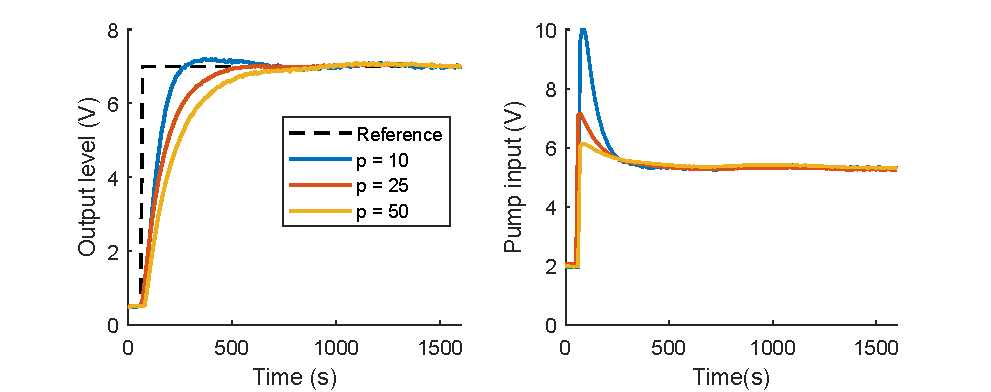
\includegraphics[width=1\textwidth]{Chapter11_ControlStudy/CoupledTanksStepResponse.pdf}
\caption{Comparison of step responses (left) for varying prediction horizon in Volterra-Laguerre MPC applied to the coupled tanks, and the corresponding MPC inputs (right)}
\label{fig:CoupledTanksStepResponse}
\end{figure}

\subsubsection{Disturbance rejection}

The addition of an output disturbance model to the MPC algorithm allowed steady-state tracking of constant reference signals in the previous two experiments, by tracking and compensating for any model errors. However, the model can also be used to reject physical disturbances such as an additional water flow from the disturbance pump (right side of Figure \ref{fig:CoupledTanksSchematic}). Using the identified 3\textsuperscript{rd} order Volterra-Laguerre model, MPC is applied to the coupled tanks at a constant 3V reference, and a 2V pulse is applied to the disturbance pump to test disturbance rejection properties. In Figure \ref{fig:CoupledTanksDisturbance}, the disturbance pulse is plotted alongside the corresponding controlled outputs for three values of the prediction horizon.

\begin{figure}[h]
\centering
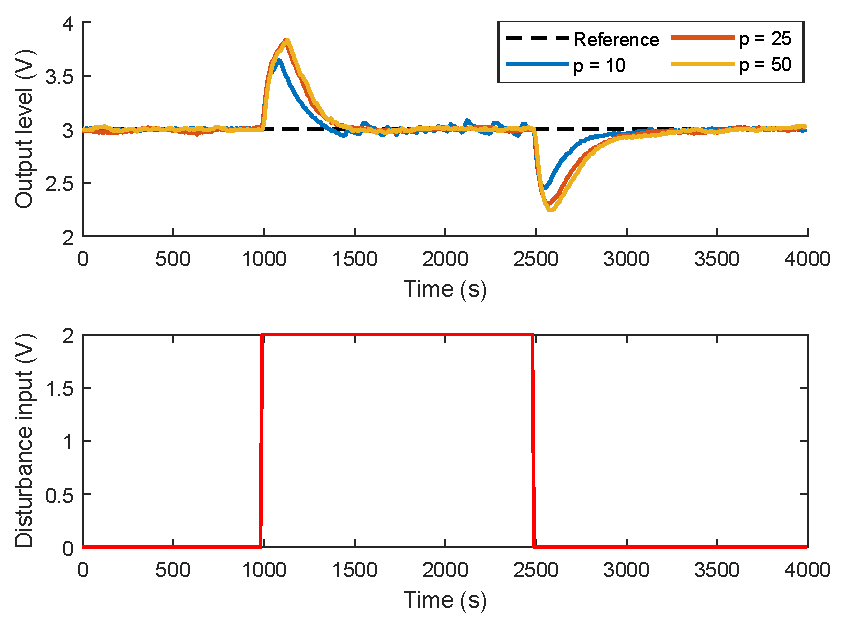
\includegraphics[width=0.9\textwidth]{Chapter11_ControlStudy/CoupledTanksDisturbance.pdf}
\caption{MPC outputs (top) for the coupled tanks system during a pulse on the disturbance pump (bottom)}
\label{fig:CoupledTanksDisturbance}
\end{figure}

The MPC scheme successfully compensates for the disturbance when it enters, and returns to normal operation after the disturbance pulse ends. The results in Figure \ref{fig:CoupledTanksDisturbance} reveal that the prediction horizon will affect the total deviation from the reference, since a lower value of $p$ provides a more aggressive response.

\section{Conclusion}

The identification and MPC methods proposed in this thesis have provided the necessary tools to enable model-based control using high order Volterra-Laguerre models. Despite the multidimensional complexity of such models, MPC was applied effectively and efficiently in this chapter to the problem of water level tracking in nonlinear tank systems. Both experimentally and in simulation, the proposed Volterra-Laguerre MPC was shown to produce desirable results in reference tracking and disturbance rejection, with significant improvements compared to control using linearized and simplified model structures. 